% Created 2023-02-28 Tue 13:22
% Intended LaTeX compiler: pdflatex
\documentclass[presentation]{beamer}
\usepackage[utf8]{inputenc}
\usepackage[T1]{fontenc}
\usepackage{graphicx}
\usepackage{longtable}
\usepackage{wrapfig}
\usepackage{rotating}
\usepackage[normalem]{ulem}
\usepackage{amsmath}
\usepackage{amssymb}
\usepackage{capt-of}
\usepackage{hyperref}
\usetheme[progressbar=foot]{metropolis}
\usetheme{metropolis}
\usecolortheme{}
\usefonttheme{}
\useinnertheme{}
\useoutertheme{}
\author{Andrew Jensen}
\date{March 9, 2023}
\title{Joint Track Machine Learning}
\hypersetup{
 pdfauthor={Andrew Jensen},
 pdftitle={Joint Track Machine Learning},
 pdfkeywords={},
 pdfsubject={},
 pdfcreator={Emacs 28.1 (Org mode 9.6)}, 
 pdflang={English}}
\usepackage{biblatex}
\addbibresource{/home/andrew/repo/lit-review/src/myBib.bib}
\addbibresource{~/org/biblio.bib}
\begin{document}

\maketitle
\begin{frame}{Outline}
\tableofcontents
\end{frame}


\section{Introduction}
\label{sec:orgf3ea1bf}
\begin{frame}[label={sec:org87094b2}]{Two columns}
\begin{columns}
\begin{column}{0.4\columnwidth}
\begin{itemize}
\item this slide consists of two columns
\item the first (left) column has no heading and consists of text
\item the second (right) column has an image and is enclosed in an
@example@ block
\end{itemize}
\end{column}
\begin{column}{0.6\columnwidth}
\begin{center}
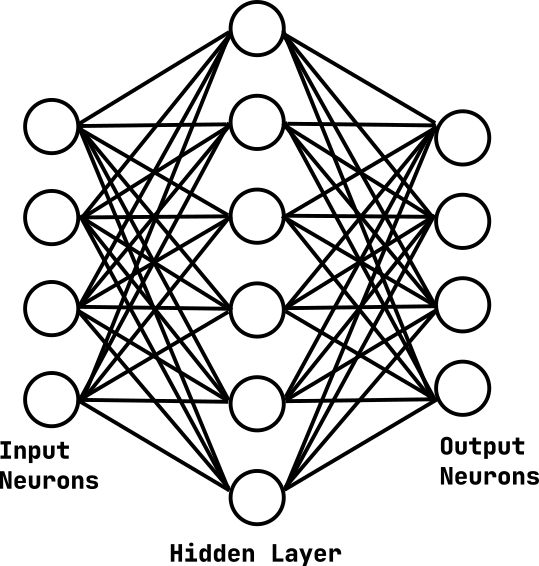
\includegraphics[width=\textwidth]{/home/andrew/repo/lit-review/figures/raster/fcn.png}
\end{center}
\end{column}
\end{columns}
\end{frame}
\begin{frame}[label={sec:org79e39eb}]{Another frame here}
Typing some things here that relate to the research.

\begin{equation*}
  T = F(s,\theta)
\end{equation*}
\end{frame}

\section{Motivation}
\label{sec:orgbfe40f4}
\begin{frame}[label={sec:orgb8cf0ac}]{The Problem}
\begin{columns}
\begin{column}{0.5\columnwidth}
\begin{itemize}
\item Joints manifest pain during dynamic activity.
\item 20\% of patients receiving TKA are dissatisfied.
\begin{itemize}
\item Instability, pain, unnatural \autocites{bakerRolePainFunction2007}[][]{bournePatientSatisfactionTotal2010}[][]{scottPredictingDissatisfactionFollowing2010}.
\end{itemize}
\item No reliable method of clinically assessing and quantifying joint dynamics.
\begin{itemize}
\item Too much human supervision, too time consuming
\end{itemize}
\end{itemize}
\end{column}
\begin{column}{0.5\columnwidth}
\begin{center}
\includegraphics[width=\textwidth]{/home/andrew/repo/lit-review/figures/raster/Physical_Examination_of_the_knee.jpg}
\end{center}
\end{column}
\end{columns}
\end{frame}
\begin{frame}[label={sec:orgc6626b1}]{Our Proposition}
\begin{columns}
\begin{column}{0.5\columnwidth}
Orthopaedic surgeons and clinicians would readily adopt a practical and inexpensive technology that allows them to measure a patient's knee kinematics during activities of daily living.
\end{column}
\begin{column}{0.55\columnwidth}
PICTURE HERE WITH RX OF KNEE MOTION STUDY
\end{column}
\end{columns}
\end{frame}
\begin{frame}[label={sec:org30c8b99}]{Constraints}
\begin{columns}
\begin{column}{0.45\columnwidth}
\begin{itemize}
\item It must fit within a standard clinical workflow
\item The technology must utilize equipment commonly found in hospitals
\item There must not be significant human supervision nor interaction to generate an examination report.
\end{itemize}
\end{column}
\begin{column}{0.55\columnwidth}
\begin{center}
\includegraphics[width=\textwidth]{/home/andrew/repo/lit-review/figures/raster/c-arm-fluoro-machine.jpg}
\end{center}
\end{column}
\end{columns}
\end{frame}
\section{Background}
\label{sec:org834e616}
\begin{frame}[label={sec:org27ac9db}]{Projective Geometry}
\end{frame}
\begin{frame}[label={sec:org9188a9b}]{Camera Intrinsics}
\end{frame}
\begin{frame}[label={sec:orgc696f3f}]{Model-Image Registration}
\end{frame}

\section{Historical Methods}
\label{sec:org54f4bf4}
\begin{frame}[label={sec:org7fbe41e}]{Overview}
Many different approaches have attempted to solve the model-image registration problem.
\begin{itemize}
\item Pre-computed projections
\item Skin-mounted motion Capture
\item Biplane Imaging
\item Iterative Projections
\end{itemize}
\end{frame}
\begin{frame}[label={sec:org46401c2}]{Pre-Computed Projections}
\end{frame}
\begin{frame}[label={sec:org9cac4da}]{Skin-mounted Motion Capture}
\end{frame}
\begin{frame}[label={sec:orgf25771e}]{Biplane Imaging}
\end{frame}
\begin{frame}[label={sec:org7f96c1d}]{Iterative Projections}
\end{frame}
\begin{frame}[label={sec:org7986f53}]{Model-based Radiostereo Photogrammetry (MBRSA)}
\end{frame}
\section{Aims}
\label{sec:org9340308}


\section{References}
\label{sec:orge201e70}
\begin{frame}[label={sec:orgcfc2455},fragile, allowframebreaks, label=]{References}
\AtNextBibliography{\tiny}
\printbibliography
\end{frame}
\end{document}